\documentclass[a4paper, 12pt]{article}

\usepackage{amsmath}
\usepackage{amssymb}
\usepackage{multirow}
\usepackage{multicol}
\usepackage{fullpage}
\usepackage{graphicx}
\usepackage{amsthm}
\usepackage{float}
\usepackage{imakeidx}
\usepackage[nottoc,numbib]{tocbibind}

\title{CS251: Assignment 7 - Question 4}
\author{Anuj Nagpal - 14116}
\date{\today}

\makeindex

\begin{document}

\maketitle
\tableofcontents
\newpage
\listoffigures
\newpage

\section{Sample Space and Random Variable}
Let $\chi$ be a \index{Random Variable}random variable such that,\\
$\chi$ : \index{Outcome}Outcome of roll of the die.\\
$\therefore \chi = \omega$ , such that $\omega \epsilon \text{\{1,2,3,4,5,6\}}$. 

\section{Probability Function of the dices}
\index{Probability Function}
\subsection{Die:1}
\[
P(\chi = x)= 
\begin{cases} 
      \frac{1}{6} & x\epsilon\text{\{1,2,3,4,5,6\}} \\
   \end{cases}
\]

\subsection{Die:2}
\[
P(\chi = x)= 
\begin{cases} 
      \frac{1}{6}-0.025 & x\epsilon\text{\{1,2,3,4\}} \\
      \frac{1}{6}+0.05 & x\epsilon\text{\{5,6\}}
   \end{cases}
\]

\subsection{Die:3}
\[
P(\chi = x)= 
\begin{cases} 
      \frac{1}{6}-0.05 & x\epsilon\text{\{1,2,3,4\}} \\
      \frac{1}{6}+0.10 & x\epsilon\text{\{5,6\}}
   \end{cases}
\]

\section{Expected Values of the Sums of the Three Dices}
\index{Expectation}
\subsection{Die:1}
E($\chi$)=$\sum_{x_{i}}P(\chi = x_{i})x_{i} = \frac{1}{6}(1+2+3+4+5+6)$ = 3.5

\subsection{Die:2}
E($\chi$)=$\sum_{x_{i}}P(\chi = x_{i})x_{i} = (\frac{1}{6}-0.025)(1+2+3+4) + (\frac{1}{6}+0.05)(5+6)$ = 3.8

\subsection{Die:3}
E($\chi$)=$\sum_{x_{i}}P(\chi = x_{i})x_{i} = (\frac{1}{6}-0.05)(1+2+3+4) + (\frac{1}{6}+0.10)(5+6)$ = 4.1

\newpage

\section{Observations}
\index{Observations}
After rolling the three dice(each die is rolled twice), it was observed that sum on Die:1 was least and sum on Die:3 was highest, i.e., we get successively higher sums for later dice.\\
This can clearly be seen in Figure~\ref{fig:figure1}.

\begin{figure}[ht]\centering
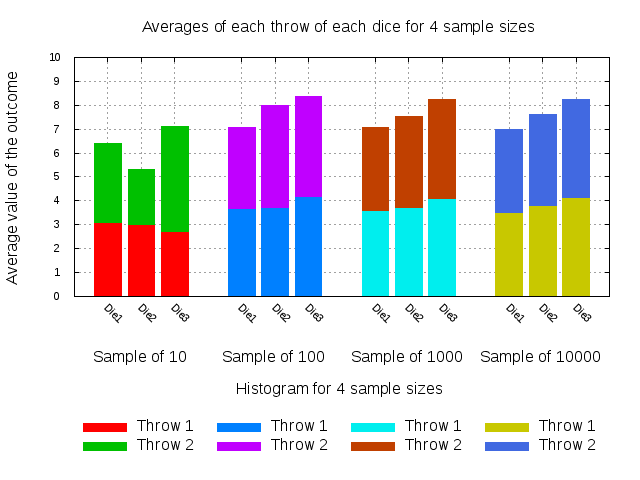
\includegraphics[width=1\columnwidth]
{output2.png}
\caption{Representation of average of each throw of all the Dice}
\label{fig:figure1}
\end{figure}

\subsection{Explanation}
\index{Explanation}
Given below are the two possible explanations of the phenomenon observed above.

\subsubsection{A Mathematical Explanation}
It is clear from the expected value of $\chi$ for all the three dices that if the experiment is repeated a large number of times, the average value of outcome would be close to the expected value. Since, the expected value is lowest for Die:1 and highest for Die:3, so, we get successively higher sums for later dice.

\subsubsection{An Intuitive Explanation}   
Since, all the outcomes on the first die are equally likely while the second die is biased in the favour of the outcomes 5 and 6 by 5\%, so, outcome of the second die was more biased to 5 and 6 which are the highest outcomes of the die. This results in a higher sum of the outcome of the second die as compared to first.\\
Now, third die is biased in the favour of the outcomes 5 and 6 by 10\%, so, outcome of the third die is biased more in the favour of 5 and 6 as compared to the second die. This results in a higher sum of the outcome of the third die as compared to second.  

\begin{figure}[ht]\centering
\includegraphics[width=0.5\columnwidth]
{q3.pdf}
\caption{Two Sample Dices}
\label{fig:figure2}
\end{figure}

\printindex

\end{document}
